
\subsection{The Theory of Hurricanes}
\label{sec:hurr-theory}

\label{sec:cyclogenesis}
TCs are a finite amplitude instability created by
wind induced sea heat exchange (WISHE);
although there is a thermodynamic disequilibrium between the tropical sea
surface and the atmosphere TCs cannot spontaneously emerge. There is
a clear separation between a tropical storm and a TC
in frequency of occurrence against maximum intensity~\cite{emanuel2005divine}.


\label{sec:carnot}


\begin{figure}
\centering
    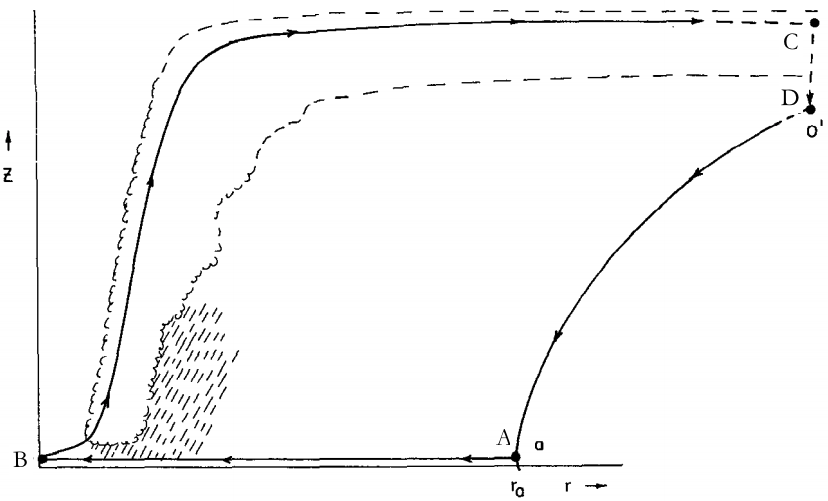
\includegraphics[width=\linewidth]{images/hurricane-carnot.png}\\
    \textit{Figure 1 from~\cite{emanuel1991theory}. }
    \caption{An idealised Carnot cycle where air parcels travel clockwise:
            A$\rightarrow$B travelling isothermally inwards into the eye-wall extracting enthalpy
            from the sea, and gaining entropy through kinetic energy dissipation;
            B$\rightarrow$C moist adiabatically thrust up into the stratosphere
            at the eye-wall and out to some some subsidence point;
            C$\rightarrow$D initial isothermal descent, albeit with some loss through radiation;
            D$\rightarrow$A final moist adiabatic descent~\cite{emanuel2018progress}. }
            \label{fig:hurricane-carnot}

\end{figure}


\begin{figure}
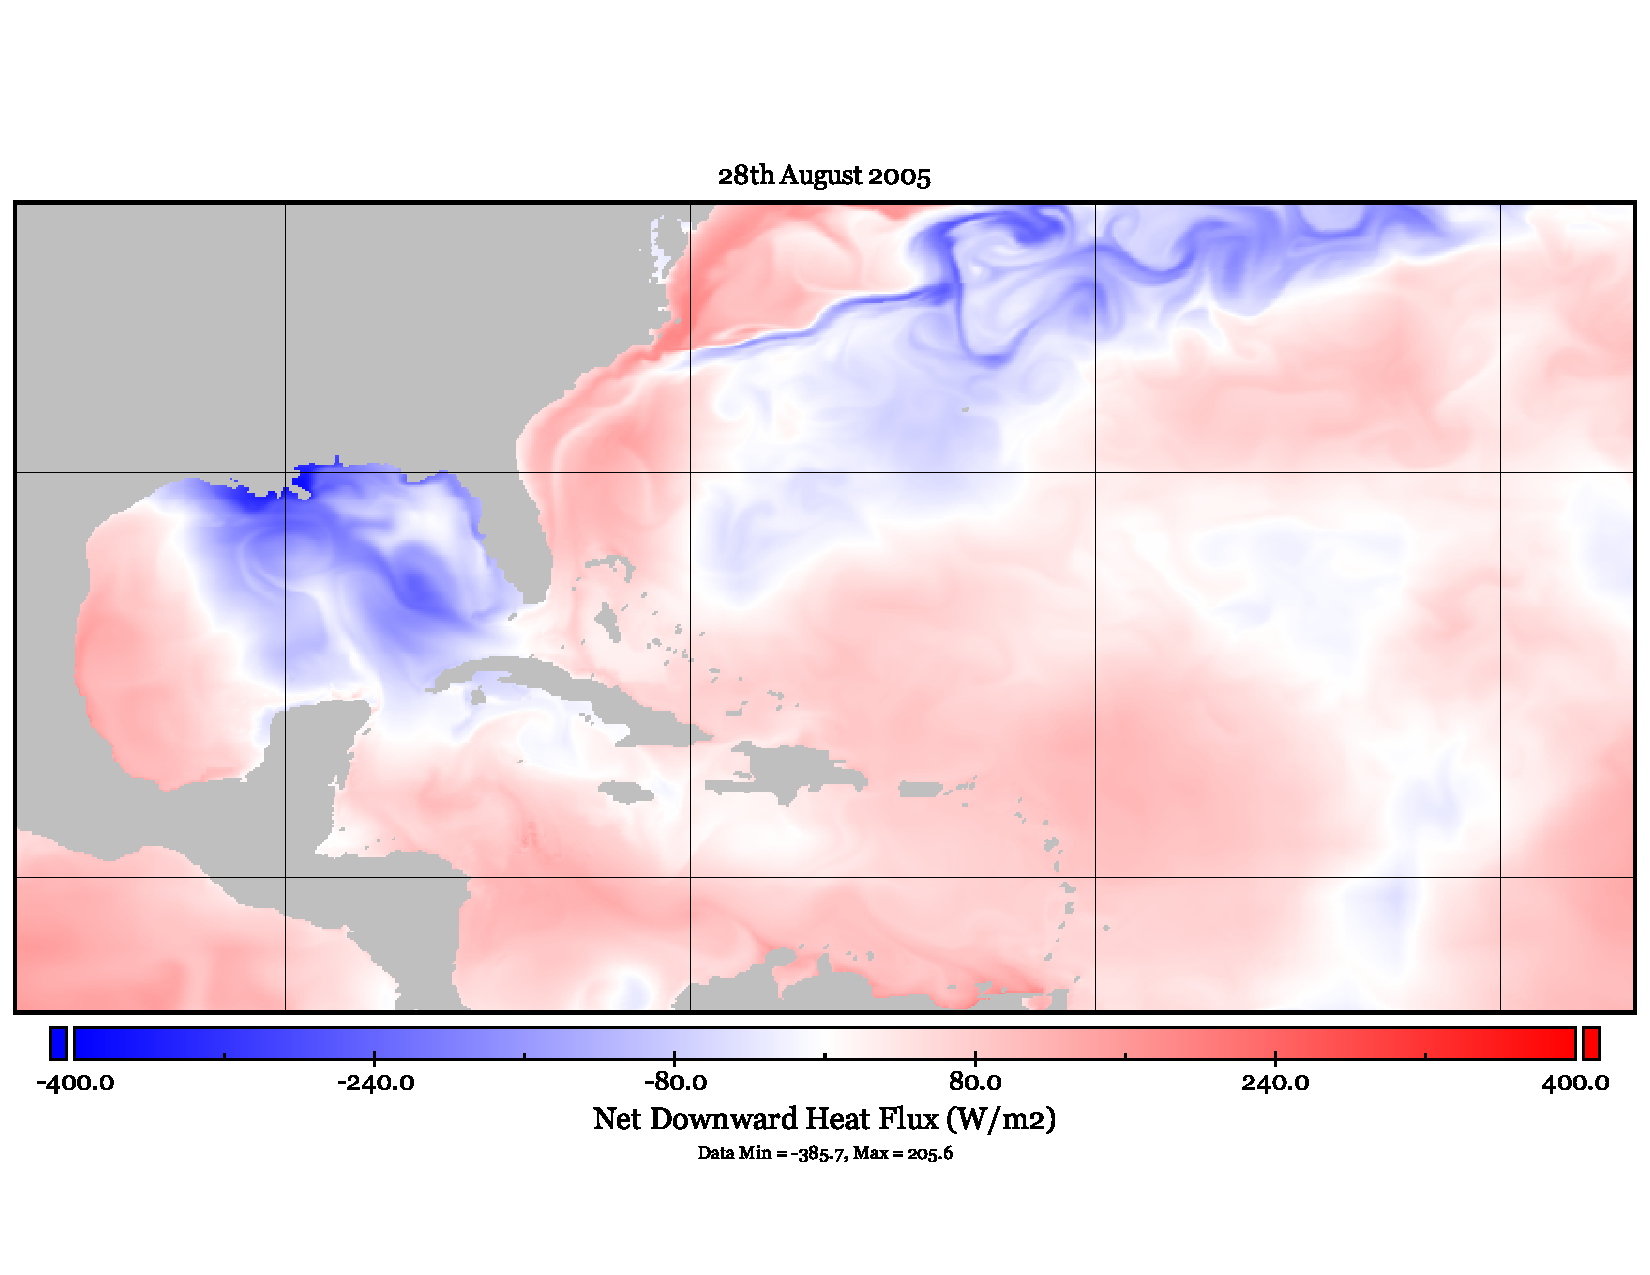
\includegraphics[width=\linewidth]{kat-heat.pdf}
\caption{The daily downwards heat flux at the sea surface on the 28th August 2005
       from \texttt{tyr}.
       The atmosphere extracts heat from the sea surface
       in the Gulf of Mexico as Katrina
       begins to make landfall. Top right shows heating of the atmosphere by
       the gulf stream (combined with an EC). }
\label{fig:heat}
\end{figure}


TCs are approximately driven by a Carnot cycle as in Figure~\ref{fig:hurricane-carnot}.
This was initially proposed by Kleinschmidt~1951~\cite{kleinschmidt1951grundlagen},
and then by Emanuel~1986~\cite{emanuel1986air, emanuel1987dependence, lilly1985steady,}.
This converts heat energy of the sea surface
(see Figure~\ref{fig:heat}) into
mechanical energy of the winds, doing the majority of the work against the sea surface,
 where near the coast it can raise a storm surge.
 The minimum central pressure (equation 26 in \cite{emanuel1986air}) is
 shown in Figure~\ref{fig:emanuel87}\footnote{Automatically updated version: \url{http://wxmaps.org/pix/hurpot}.}
 to closely match the measured
minimum central pressure of the largest storms.
The potential intensity is conventionally viewed through the
maximum windspeed (equation 15-7 in \cite{emanuel2018progress}) is,

\begin{equation}
\left|\mathbf{V}_{s}\right|^{2}=\frac{C_{k}}{C_{D}}
\frac{T_{s}-T_{o}}{T_{o}}\left(k_{0}^{*}-k_b\right),
\tag{PI}
\label{eq:PI}
\end{equation}

where $C_d$ is the surface drag coefficient $C_k$ is the
 enthalpy surface exchange coefficient.
$T_s$ is the sea surface temperature ($K$), $T_o$ is the temperature of the
tropopause at the end of the moist adiabatic rise ($K$), $T_b$ is
the temperature at the top of the planetary boundary layer.
One can see that the a warmer sea surface, and a cooler lower stratosphere
would both lead to a higher potential intensity
(§~\ref{sec:1d-hurr})~\cite{emanuel1991theory, emanuel2018progress}.
In \ref{eq:PI} the enthalpy per unit mass, $k$,
(equation 15-8 in \cite{emanuel2018progress}) is

\begin{equation}
k \equiv c_{p} T +L_{v} q,
\label{eq:enthalpy_per_unit_mass}
\end{equation}



where $c_p$ is the heat capacity at constant pressure and $L_{v}$ is the latent heat
of vaporisation. $k_{0}^{*}$ is the saturation enthalpy at the sea
surface~\cite{emanuel2018progress}.%\footnote{
%There is a positive feedback loop from air cooling adiabatically as it flows down
%the pressure gradient, and therefore increasing the enthalpy disequilibrium
%$k_{0}^{*}-k$, leading to a root below 700 mbar central pressure called a `hypercane'~\cite{emanuel1987dependence}
%where dissipation of energy in areas apart from the sea surface must become important.

%}

\begin{figure}[htb!]
\centering
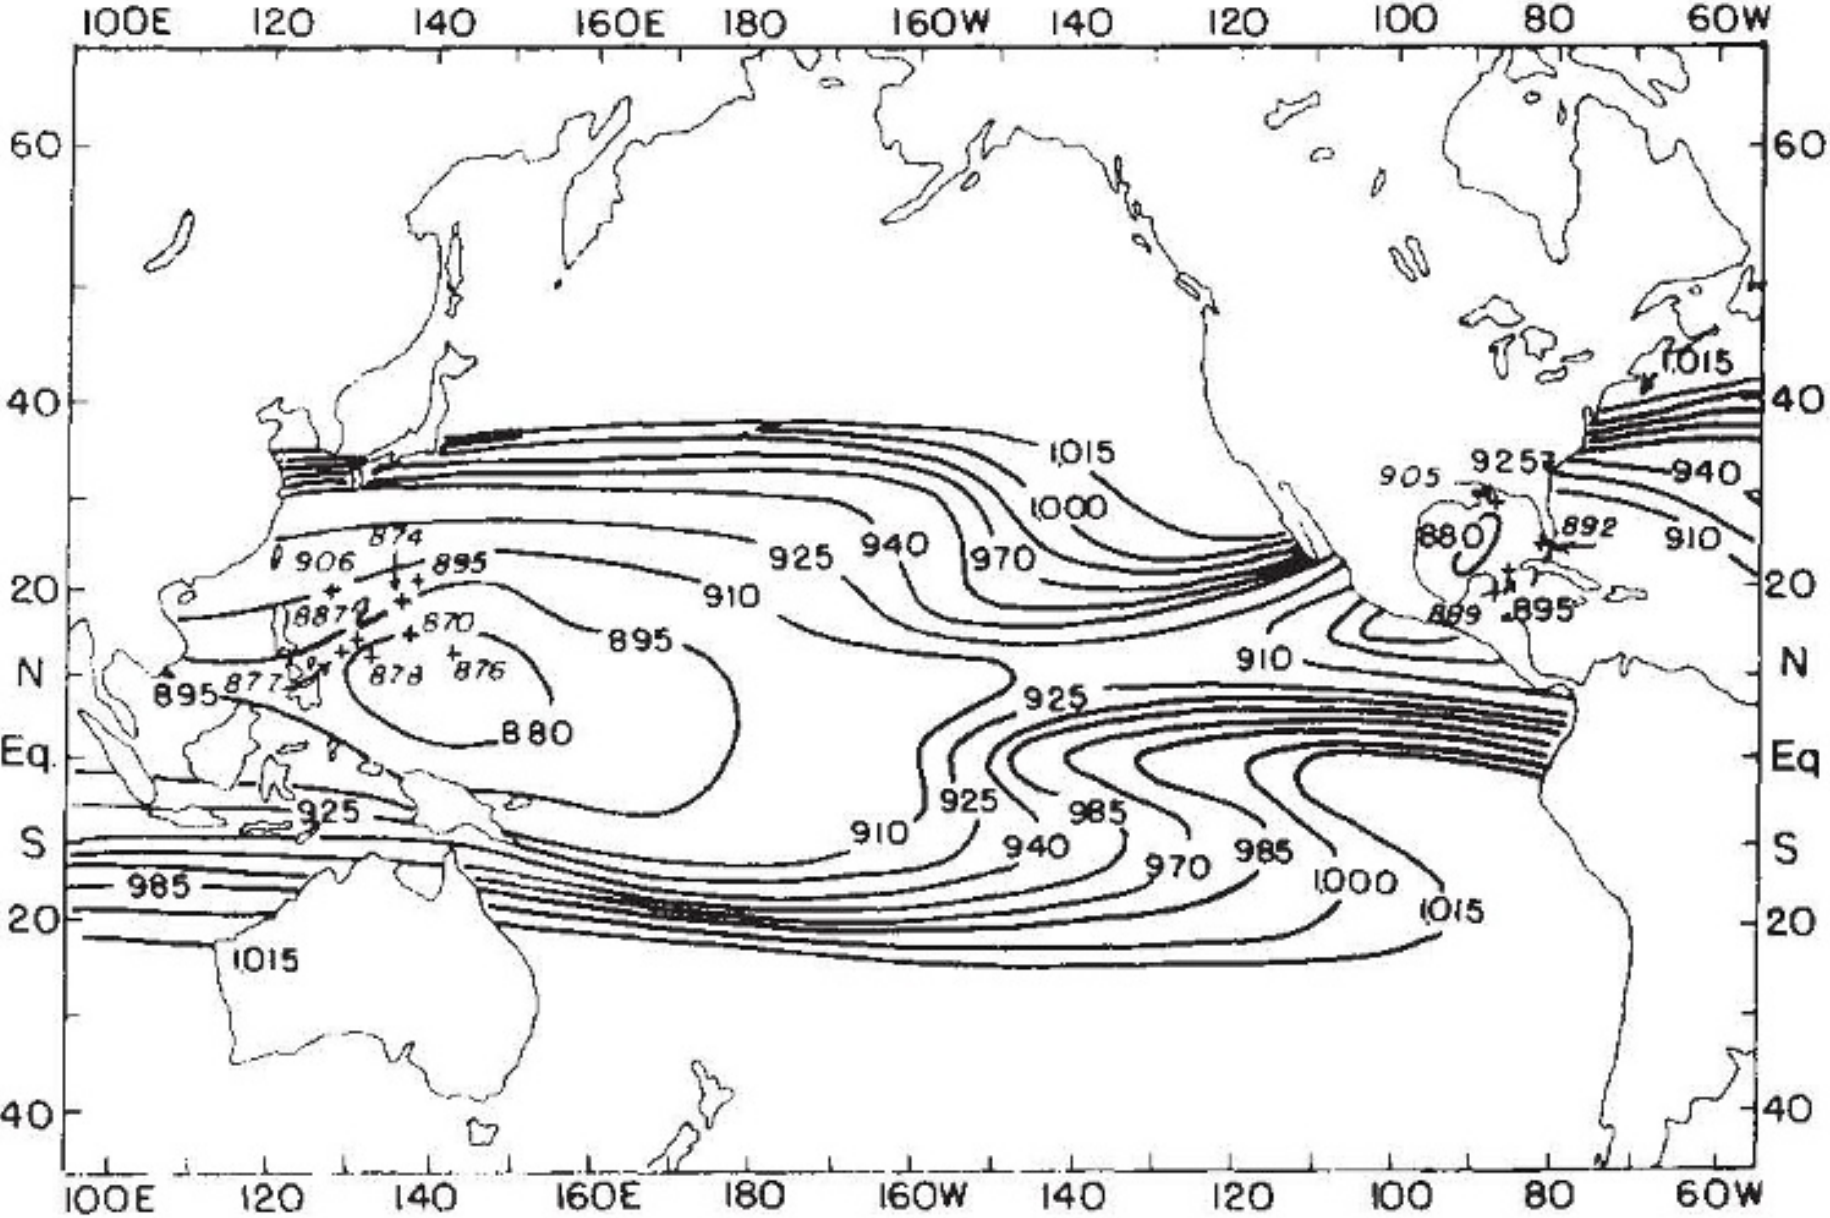
\includegraphics[width=1\linewidth]{images/e87-slimmed-verif.png}\\
\textit{Figure 2 from Emanuel, Nature, 1987~\cite{emanuel1987dependence}}
\caption{minimum sustainable central pressures (mb) under September mean
climatological conditions, assuming an ambient pressure of 1,015 mb~\cite{emanuel1986air}.
Crosses mark the positions and central pressures of some of the most intense
tropical cyclones on record~\cite{anthes2016tropical}.
The data shows that at the time the minimum central pressure
closely matches the limits predicted~\cite{emanuel1986air}. }
\label{fig:emanuel87}
\end{figure}




Most TCs do not reach their PI.
One reason for this is that
water column is only at the surface temperature
to some depth (the mixed layer depth), and colder below.
The majority of the cooling of
the sea surface during a TC occurs due to the
upwards mixing of this colder water.
The warm water
is much deeper at the western boundary currents~\cite{hogg1995western},
which means that if a TC
travels down the axis of the current (e.g.~the loop current)
it can reach a higher intensity than
if it travelled 20km to one side~\cite{emanuel2005divine}.
